\documentclass[11pt,a4paper]{article}

% --- Språk & typografi ---
\usepackage[T1]{fontenc}
\usepackage[utf8]{inputenc}
\usepackage[swedish]{babel}
\usepackage{lmodern}
\usepackage{microtype}
\usepackage{tikz}

% --- Layout ---
\usepackage{geometry}
\geometry{margin=22mm}
\setlength{\parindent}{0pt}
\setlength{\parskip}{6pt}

% --- Rubriker & sidhuvud ---
\usepackage{titlesec}
\usepackage{fancyhdr}
\pagestyle{fancy}
\fancyhf{}
\lhead{MVE655 — Teorilista (övningsmall)}
\rhead{\thepage}
\renewcommand{\headrulewidth}{0.4pt}

% --- Länkar (valfritt, men bra för TOC) ---
\usepackage[hidelinks]{hyperref}

% --- Boxar för svar ---
\usepackage{xcolor}
\usepackage[most]{tcolorbox}
\tcbset{
  colback=gray!3,
  colframe=gray!35,
  boxrule=0.6pt,
  arc=2mm,
  left=2.5mm,right=2.5mm,top=2mm,bottom=2mm,
  breakable
}

\newtcolorbox{AnswerBox}[2][]{%
  title={#2},
  #1
}

% --- Små “metadata”-rader ---
\newcommand{\Kalla}[1]{\textit{\small Källa: #1}\par\vspace{2mm}}

% --- Makron för olika typer av uppgifter ---
\newcommand{\DefItem}[2]{%
  \subsubsection*{#1}%
  \Kalla{#2}%
  \begin{AnswerBox}{Ditt svar (definition + ev. exempel/kommentar)}%
  \vspace{5.0cm}
  \end{AnswerBox}\vspace{2mm}
}

\newcommand{\ThmItem}[2]{%
  \subsubsection*{#1}%
  \Kalla{#2}%
  \begin{AnswerBox}{Ditt svar (satsens formulering)}%
  \vspace{5.5cm}
  \end{AnswerBox}\vspace{2mm}
}

\newcommand{\ProofItem}[2]{%
  \subsubsection*{#1}%
  \Kalla{#2}%
  \begin{AnswerBox}{Formulering}%
  \vspace{3.8cm}
  \end{AnswerBox}\vspace{2mm}
  \begin{AnswerBox}{Bevis / motivering (struktur + nyckelsteg)}%
  \vspace{8.0cm}
  \end{AnswerBox}\vspace{2mm}
}

% --- Titel ---
\title{\vspace{-6mm}Teorilista – tentamall i \LaTeX\\
\large Flervariabelkursen MVE655, läsåret 2025/26}
\date{}

\begin{document}
\maketitle
\vspace{-2mm}

\tableofcontents
\vspace{2mm}
\hrule
\vspace{4mm}

% ============================================================
\section{Definiera}

\subsection{Grundbegrepp i $\mathbb{R}^n$ och mängdlära/topologi}
\subsubsection*{Avståndet mellan två punkter i $\mathbb{R}^n$}
\Kalla{föreläsning 1 (se även sid 2,6,7 för $n=1,2,3$)}
\begin{AnswerBox}{Definition + exempel}
Avstandet mellan $x,y\in\mathbb{R}^n$ ar $|x-y|=\sqrt{(x_1-y_1)^2+\dots+(x_n-y_n)^2}$. Exempel: i $\mathbb{R}^2$ ar $|(1,0)-(0,1)|=\sqrt{2}$.
\end{AnswerBox}\vspace{2mm}

\subsubsection*{Omgivning till en punkt i $\mathbb{R}^n$}
\Kalla{föreläsning 2 (se även sid 4,7,9 för $n=1,2,3$)}
\begin{AnswerBox}{Definition + exempel}
En (oppna) omgivning till $a\in\mathbb{R}^n$ ar en boll $B_r(a)=\{x:|x-a|<r\}$ for nagot $r>0$. Exempel: $B_1(0)$ ar enhetsbollen.
\end{AnswerBox}\vspace{2mm}

\subsubsection*{Inre punkt, yttre punkt och randpunkt till en mängd i $\mathbb{R}^n$}
\Kalla{föreläsning 2 (se även sid 4,8 för $n=1,2$)}
\begin{AnswerBox}{Definition + exempel}
En inre punkt $a\in A$ har en boll $B_r(a)\subset A$. En yttre punkt har en boll utan intersection med $A$. En randpunkt ar en punkt vars varje boll innehaller bade punkter i $A$ och i komplementet. Exempel: For intervallet $(0,1)$ i $\mathbb{R}$ ar alla punkter i $(0,1)$ inre, alla utanfor yttre och $0,1$ randpunkter.
\end{AnswerBox}\vspace{2mm}

\subsubsection*{Öppen, sluten, begränsad och kompakt mängd i $\mathbb{R}^n$}
\Kalla{föreläsning 2 (se även sid 9 för $n=2$)}
\begin{AnswerBox}{Definition + exempel}
$A$ ar oppen om varje punkt ar inre. $A$ ar sluten om den innehaller alla sina randpunkter (equiv. komplementet ar oppet). $A$ ar begransad om $A\subset B_R(0)$ for nagot $R$. $A$ ar kompakt om det ar slutet och begransat (Heine-Borel). Exempel: Den slutna enhetsbollen $B_1(0)$ ar kompakt.
\end{AnswerBox}\vspace{2mm}

\subsection{Grafer och nivåmängder}
\subsubsection*{Graf och nivåkurva för en funktion från $\mathbb{R}^2$ till $\mathbb{R}$}
\Kalla{sid 57 \& 59, eller föreläsning 3}
\begin{AnswerBox}{Definition + exempel}
Grafen till $f(x,y)$ ar $\{(x,y,f(x,y))\}\subset\mathbb{R}^3$. En nivakurva for niv\aa\ $c$ ar $\{(x,y):f(x,y)=c\}$. Exempel: For $f(x,y)=x^2+y^2$ ar nivakurvorna cirklar.
\end{AnswerBox}\vspace{2mm}

\subsubsection*{Nivåyta till en funktion från $\mathbb{R}^3$ till $\mathbb{R}$}
\Kalla{sid 63, eller föreläsning 4}
\begin{AnswerBox}{Definition + exempel}
En niv\aa yta ar $\{(x,y,z):f(x,y,z)=c\}$. Exempel: For $f(x,y,z)=x^2+y^2+z^2$ ar nivoytorna sfarer av radie $\sqrt{c}$.
\end{AnswerBox}\vspace{2mm}

\subsection{Gränsvärden och kontinuitet}
\subsubsection*{Gränsvärde av en funktion från $\mathbb{R}^n$ till $\mathbb{R}^m$}
\Kalla{föreläsning 4 (se även sid 81 för $n=2,m=1$)}
\begin{AnswerBox}{Definition + skiss}
\textbf{Definition.} En funktion $f:\mathbb{R}^n \to \mathbb{R}^m$ har gränsvärdet $A \in \mathbb{R}^m$ i punkten $a \in \mathbb{R}^n$ om det för alla $\varepsilon > 0$ existerar $\delta > 0$ s.a.
\[
|f(x)-A| < \varepsilon, \quad \text{för alla } x \in D_f \text{ s.a. } 0 < |x-a| < \delta.
\]
Detta skrivs $\lim_{x\to a} f(x)=A$ eller $f(x)\to A$ då $x \to a$.

\begin{center}
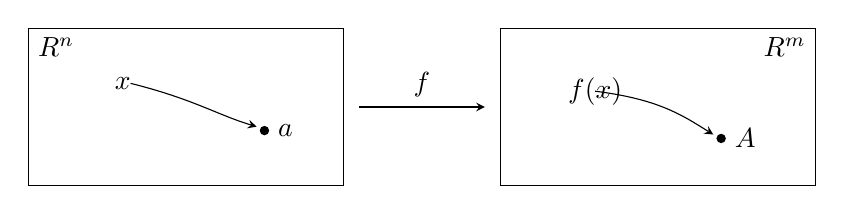
\begin{tikzpicture}[>=stealth]
  \draw (0,0) rectangle (4,2);
  \node[anchor=north west] at (0,2) {$\mathbb{R}^n$};
  \node at (1.2,1.3) {$x$};
  \draw[->] (1.3,1.3) .. controls (2.1,1.1) and (2.4,0.9) .. (2.9,0.75);
  \node[circle, fill, inner sep=1.2pt] at (3.0,0.7) {};
  \node[anchor=west] at (3.05,0.7) {$a$};

  \draw (6,0) rectangle (10,2);
  \node[anchor=north east] at (10,2) {$\mathbb{R}^m$};
  \node at (7.2,1.2) {$f(x)$};
  \draw[->] (7.2,1.2) .. controls (8.0,1.1) and (8.3,0.9) .. (8.7,0.65);
  \node[circle, fill, inner sep=1.2pt] at (8.8,0.6) {};
  \node[anchor=west] at (8.85,0.6) {$A$};

  \draw[->] (4.2,1) -- (5.8,1) node[midway, above] {$f$};
  \end{tikzpicture}
\end{center}
\end{AnswerBox}\vspace{2mm}
\subsubsection*{Kontinuitet av en funktion från $\mathbb{R}^n$ till $\mathbb{R}^m$}
\Kalla{föreläsning 4 (se även sid 89 för $n=2,m=1$)}
\begin{AnswerBox}{Definition + kommentar}
$f$ ar kontinuerlig i $a$ om $\lim_{x\to a}f(x)=f(a)$, dvs. for alla $\varepsilon>0$ finns $\delta>0$ s.a. $|x-a|<\delta$ ger $|f(x)-f(a)|<\varepsilon$. $f$ ar kontinuerlig om den ar kontinuerlig i alla punkter i definitionsmangden.
\end{AnswerBox}\vspace{2mm}

\subsection{Derivator, differentierbarhet och linjär algebra för avbildningar}
\subsubsection*{Partiell derivata för en funktion från $\mathbb{R}^2$ till $\mathbb{R}$}
\Kalla{sid 94, eller föreläsning 5}
\begin{AnswerBox}{Definition + exempel}
Partiell derivata med avseende pa $x$ i punkten $(a,b)$: $f_x(a,b)=\lim_{h\to 0}\frac{f(a+h,b)-f(a,b)}{h}$ (analogt for $f_y$). Exempel: $f(x,y)=x^2y$ ger $f_x=2xy$, $f_y=x^2$.
\end{AnswerBox}\vspace{2mm}

\subsubsection*{Differentierbarhet för en funktion från $\mathbb{R}^2$ till $\mathbb{R}$}
\Kalla{föreläsning 6 (obs! bokens definition på sid 103 skiljer sig något)}
\begin{AnswerBox}{Definition + kommentar}
$f$ ar differentierbar i $(a,b)$ om det finns en linjar avbildning (gradienten) sa att
\[
f(a+h,b+k)=f(a,b)+f_x(a,b)h+f_y(a,b)k+o\left(\sqrt{h^2+k^2}\right).
\]
Da ar gradienten $\nabla f(a,b)=(f_x(a,b),f_y(a,b))$.
\end{AnswerBox}\vspace{2mm}

\subsubsection*{Funktionalmatris/Jacobimatris för en funktion från $\mathbb{R}^n$ till $\mathbb{R}^m$}
\Kalla{sid 190, eller föreläsning 6}
\begin{AnswerBox}{Definition}
Jacobimatrisen $J_f(a)$ har element $(\partial f_i/\partial x_j)(a)$, dvs.
\[
J_f(a)=
\begin{bmatrix}
\frac{\partial f_1}{\partial x_1} & \dots & \frac{\partial f_1}{\partial x_n}\\
\vdots & & \vdots\\
\frac{\partial f_m}{\partial x_1} & \dots & \frac{\partial f_m}{\partial x_n}
\end{bmatrix}_{x=a}.
\]
\end{AnswerBox}\vspace{2mm}

\subsubsection*{Linjärisering av en funktion från $\mathbb{R}^n$ till $\mathbb{R}^m$}
\Kalla{föreläsning 6 (obs! boken använder begreppet annorlunda; båda tolkningar rätt)}
\begin{AnswerBox}{Definition}
Den linjara approximationen i $a$ ar $L(h)=f(a)+J_f(a)\,h$. For sma $h$ ar $f(a+h)\approx L(h)$.
\end{AnswerBox}\vspace{2mm}

\subsection{Gradient och riktningsderivata}
\subsubsection*{Gradienten av en funktion från $\mathbb{R}^n$ till $\mathbb{R}$}
\Kalla{föreläsning 8 (se sid 99 för $n=2$)}
\begin{AnswerBox}{Definition + tolkning}
\[
\nabla f(x)=\left(\frac{\partial f}{\partial x_1}(x),\dots,\frac{\partial f}{\partial x_n}(x)\right).
\]
Den pekar i brantaste uppforbackens riktning; $|\nabla f|$ ar stigningshastigheten dar.
\end{AnswerBox}\vspace{2mm}
\subsubsection*{Riktningsderivata av en funktion från $\mathbb{R}^n$ till $\mathbb{R}$}
\Kalla{föreläsning 8 (se sid 101 för $n=2$)}
\begin{AnswerBox}{Ditt svar (definition + ev. exempel/kommentar)}
\textbf{Definition.} Med riktningsderivatan av $f:\mathbb{R}^n\to\mathbb{R}$ i punkten $a\in\mathbb{R}^n$ och riktningen $v$, dar $|v|=1$, menas
\[
f_v'(a)=\lim_{h\to 0}\frac{f(a+hv)-f(a)}{h}.
\]
\end{AnswerBox}\vspace{2mm}

\subsection{Optimering}
\subsubsection*{Lokalt maximum/minimum för en funktion från $\mathbb{R}^n$ till $\mathbb{R}$}
\Kalla{föreläsning 11 (se sid 150 för $n=2$)}
\begin{AnswerBox}{Definition}
$f$ har lokalt max/min i $a$ om det finns $\delta>0$ s.a. $f(x)\le f(a)$ (resp. $f(x)\ge f(a)$) for alla $x$ med $|x-a|<\delta$.
\end{AnswerBox}\vspace{2mm}

\subsubsection*{Lokal extrempunkt och lokalt extremvärde för en funktion från $\mathbb{R}^n$ till $\mathbb{R}$}
\Kalla{föreläsning 11 (se sid 151 för $n=2$)}
\begin{AnswerBox}{Definition}
Punkten $a$ kallas lokal extrempunkt (max eller min) och vardet $f(a)$ ar lokalt extremvarde.
\end{AnswerBox}\vspace{2mm}

\subsubsection*{Stationär punkt och sadelpunkt till en funktion från $\mathbb{R}^n$ till $\mathbb{R}$}
\Kalla{föreläsning 11 (se sid 152 för $n=2$)}
\begin{AnswerBox}{Definition}
Stationar punkt: $\nabla f(a)=0$. Sadelpunkt: stationar punkt som varken ar lokalt max eller min (funktion vaxlar tecken runt punkten).
\end{AnswerBox}\vspace{2mm}

\subsubsection*{Hessematris/Hessianen för en funktion från $\mathbb{R}^n$ till $\mathbb{R}$}
\Kalla{föreläsning 11}
\begin{AnswerBox}{Definition}
Hessianen i $a$ ar matrisen av andraderivator: $H_f(a)=[\partial^2 f/\partial x_i \partial x_j]_{i,j}$. Anvands for att klassificera stationara punkter.
\end{AnswerBox}\vspace{2mm}

\subsubsection*{Globalt maximum/minimum för en funktion från $\mathbb{R}^n$ till $\mathbb{R}$}
\Kalla{föreläsning 12 (se även sid 162 för begreppet global extrempunkt)}
\begin{AnswerBox}{Definition}
Globalt max/min i $a$ betyder $f(x)\le f(a)$ (resp. $\ge f(a)$) for alla $x$ i definitionsmangden. Pa kompakta mangder antar kontinuerliga funktioner globala extremvarden (Weierstrass).
\end{AnswerBox}\vspace{2mm}

\subsection{Integraler och koordinatbyten}
\subsubsection*{Riemannsumma för en funktion från $\mathbb{R}^2$ till $\mathbb{R}$}
\Kalla{sid 253, eller PowerPoint på föreläsning 13}
\begin{AnswerBox}{Definition}
Delar man ett omrade $D$ i sma rektanglar $R_{ij}$ med punkt $\xi_{ij}$ i varje, sa ar en Riemannsumma $\sum f(\xi_{ij})\,\Delta A_{ij}$. Integralen $\iint_D f$ ar gransen da finhetsgraden gar mot noll.
\end{AnswerBox}\vspace{2mm}

\subsubsection*{Sambandet mellan kartesiska och polära koordinater samt areaelement}
\Kalla{sid 46, 199, eller föreläsning 2 \& 14}
\begin{AnswerBox}{Definition + exempel}
Transform: $x=r\cos\theta$, $y=r\sin\theta$, $r\ge 0$, $\theta\in[0,2\pi)$. Areaelement: $dA=r\,dr\,d\theta$. Exempel: cirkelskiva av radie $R$ blir $0\le r\le R$, $0\le\theta<2\pi$.
\end{AnswerBox}\vspace{2mm}

\subsubsection*{Sambandet mellan kartesiska och sfäriska/rymdpolära koordinater samt volymelement}
\Kalla{sid 52, 200, eller föreläsning 2 \& 16}
\begin{AnswerBox}{Definition + kommentar}
Vanlig ordning: $x=\rho\sin\phi\cos\theta$, $y=\rho\sin\phi\sin\theta$, $z=\rho\cos\phi$ med $\rho\ge 0$, $\phi\in[0,\pi]$, $\theta\in[0,2\pi)$. Volymelement: $dV=\rho^2\sin\phi\, d\rho\, d\phi\, d\theta$.
\end{AnswerBox}\vspace{2mm}
\subsubsection*{Sambandet mellan kartesiska och cylindriska koordinater samt volymelement}
\Kalla{föreläsning 2 \& 16 (se även sid 49)}
\begin{AnswerBox}{Ditt svar (definition + ev. exempel/kommentar)}
\textbf{Cylindriska koordinater.} Sambandet ges av
\[
x=r\cos\theta,\qquad y=r\sin\theta,\qquad z=z.
\]
\textbf{Exempel.} Punkten $(-1,1,-1)$ har cylindriska koordinater
\[
\left(\sqrt{2},\frac{3\pi}{4},-1\right).
\]
\end{AnswerBox}\vspace{2mm}
\subsubsection*{Medelvärde av en reellvärd funktion av två/tre variabler på ett område}
\Kalla{föreläsning 17}
\begin{AnswerBox}{Definition}
For omrade $D$ med area/volym $|D|$ definieras medelvardet
\[
\bar{f}=\frac{1}{|D|}\iint_D f\,dA \quad (\text{eller } \bar{f}=\frac{1}{|D|}\iiint_D f\,dV).
\]
\end{AnswerBox}\vspace{2mm}

\subsection{Kurvor och kurvintegraler}
\subsubsection*{Parametrisering av en kurva}
\Kalla{sid 66 \& 67 (se även föreläsning 8 \& 18)}
\begin{AnswerBox}{Definition + exempel}
En kurva ges av $r(t)=(x(t),y(t),z(t))$, $t\in[a,b]$. Exempel: en cirkel radie $R$: $r(t)=(R\cos t,R\sin t)$, $t\in[0,2\pi]$.
\end{AnswerBox}\vspace{2mm}

\subsubsection*{Hastighet, fart och accelleration för en parametriserad rörelse}
\Kalla{föreläsning 18 (se även sid 184--185)}
\begin{AnswerBox}{Definition}
Hastighet $v(t)=r'(t)$, fart $|v(t)|$, acceleration $a(t)=r''(t)$. Fysikalisk tolkning som positions-, hastighets- och accelerationsvektorer.
\end{AnswerBox}\vspace{2mm}

\subsubsection*{Enkel, sluten, sammansatt och orienterad kurva}
\Kalla{sid 211 \& 212, eller föreläsning 18}
\begin{AnswerBox}{Definition}
Enkel: skar inte sig sjalv. Sluten: $r(a)=r(b)$. Sammansatt: styckvis definierad av flera parametriseringar. Orienterad: riktning ges av parametriseringens okande parameter.
\end{AnswerBox}\vspace{2mm}

\subsubsection*{Bågelementet för en parametriserad kurva}
\Kalla{sid 275, eller föreläsning 18}
\begin{AnswerBox}{Definition}
Differentialt bagelment $ds=|r'(t)|\,dt$. Anvands i kurvintegraler och kurvlängd.
\end{AnswerBox}\vspace{2mm}

\subsubsection*{Integralen av funktion över kurva (kurvintegral) och längden av en kurva}
\Kalla{sid 274--276, 278, eller föreläsning 18}
\begin{AnswerBox}{Definition}
Kurvlängd: $L=\int_a^b |r'(t)|\,dt$. Kurvintegral av skalart f: $\int_C f\, ds=\int_a^b f(r(t))\,|r'(t)|\,dt$.
\end{AnswerBox}\vspace{2mm}

\subsection{Vektorfält och potential}
\subsubsection*{Fältlinje till vektorfält}
\Kalla{föreläsning 19}
\begin{AnswerBox}{Definition}
Kurva $r(t)$ som uppfyller $r'(t)=F(r(t))$. Den visar riktningen for faltet.
\end{AnswerBox}\vspace{2mm}

\subsubsection*{Tangentkurvintegral (kurvintegral av vektorfält)}
\Kalla{sid 285, 328, eller föreläsning 19}
\begin{AnswerBox}{Definition}
For $F$ och kurva $C$ med parametrisering $r(t)$: $\int_C F\cdot dr=\int_a^b F(r(t))\cdot r'(t)\,dt$. Tolkning: arbete langs $C$.
\end{AnswerBox}\vspace{2mm}

\subsubsection*{Konservativt vektorfält (potentialfält) och potential}
\Kalla{sid 303, 328, 329, eller föreläsning 21}
\begin{AnswerBox}{Definition + egenskap}
$F$ ar konservativt om det finns $\phi$ med $F=\nabla\phi$. Da beror linjeintegraler bara pa andpunkter och $\int_C F\cdot dr=\phi(B)-\phi(A)$.
\end{AnswerBox}\vspace{2mm}

\subsubsection*{Enkelt sammanhängande mängd/område}
\Kalla{sid 312, 343, eller föreläsning 21}
\begin{AnswerBox}{Definition}
Omrade dar varje sluten kurva kan dras ihop till en punkt utan att lamna omradet (inga hal i 2D/3D).
\end{AnswerBox}\vspace{2mm}

\subsubsection*{Ekvipotentialkurvor till plana konservativa vektorfält}
\Kalla{föreläsning 21}
\begin{AnswerBox}{Definition}
Kurvorna $\phi(x,y)=c$ for potentialen $\phi$. Faltet ar ortogonalt mot dessa kurvor.
\end{AnswerBox}\vspace{2mm}

\subsubsection*{Ekvipotentialytor till konservativa vektorfält i rummet}
\Kalla{föreläsning 21}
\begin{AnswerBox}{Definition}
Ytor $\phi(x,y,z)=c$. Potentialfaltet $\nabla\phi$ star ortogonalt mot ytorna.
\end{AnswerBox}\vspace{2mm}

\subsection{Ytor, ytintegraler och differentialoperatorer}
\subsubsection*{Parametrisering av en yta}
\Kalla{sid 69, eller föreläsning 22}
\begin{AnswerBox}{Definition + exempel}
Yta ges av $r(u,v)=(x(u,v),y(u,v),z(u,v))$ for $(u,v)$ i ett parameteromrade. Exempel: sfaryta radie $R$: $r(\phi,\theta)=(R\sin\phi\cos\theta,R\sin\phi\sin\theta,R\cos\phi)$.
\end{AnswerBox}\vspace{2mm}

\subsubsection*{Areaelementet för en parametriserad yta}
\Kalla{sid 279, eller föreläsning 22}
\begin{AnswerBox}{Definition}
Differentialt areaelement: $dS=|r_u\times r_v|\,du\,dv$.
\end{AnswerBox}\vspace{2mm}

\subsubsection*{Integralen av funktion över yta (ytintegral) och arean av en yta}
\Kalla{sid 279, 281, eller föreläsning 22}
\begin{AnswerBox}{Definition}
Area av param yta: $\iint |r_u\times r_v|\,du\,dv$. YtIntegral av $f$: $\iint f(r(u,v))\,|r_u\times r_v|\,du\,dv$.
\end{AnswerBox}\vspace{2mm}

\subsubsection*{Orientering av yta}
\Kalla{sid 215, eller föreläsning 23}
\begin{AnswerBox}{Definition}
Val av en sammanhangande normalriktning (t.ex. utat/inat) som gor ytan orienterbar. $r_u\times r_v$ ger en vald normal.
\end{AnswerBox}\vspace{2mm}

\subsubsection*{Normalytelement för en yta}
\Kalla{föreläsning 23}
\begin{AnswerBox}{Definition}
Normalytelement $d\mathbf{S}=\hat{n}\, dS$ dar $\hat{n}$ ar enhetsnormalen (med vald orientering).
\end{AnswerBox}\vspace{2mm}

\subsubsection*{Normalytintegral/Flödesintegral (ytintegral av vektorfält)}
\Kalla{sid 332, eller föreläsning 23}
\begin{AnswerBox}{Definition}
For vektorfaltet $F$ och orienterad yta: $\iint_S F\cdot d\mathbf{S}=\iint_S F\cdot \hat{n}\, dS$ (flode genom ytan).
\end{AnswerBox}\vspace{2mm}

\subsubsection*{Divergensen och rotationen av vektorfält}
\Kalla{sid 324, 322 (plan); sid 348, 336 (rum), eller föreläsning 24}
\begin{AnswerBox}{Definition}
Divergens: $\operatorname{div}F=\nabla\cdot F$. Rotation (curl): $\operatorname{rot}F=\nabla\times F$ (i planet: $\partial Q/\partial x-\partial P/\partial y$ for $F=(P,Q)$).
\end{AnswerBox}\vspace{2mm}

\subsubsection*{Divergensfritt/Källfritt vektorfält}
\Kalla{sid 325, 354, eller föreläsning 24}
\begin{AnswerBox}{Definition}
$\operatorname{div}F=0$ i omradet. Inga kallar/sankar; flodet genom varje sluten yta ar noll.
\end{AnswerBox}\vspace{2mm}

\subsubsection*{Rotationsfritt/Virvelfritt vektorfält}
\Kalla{sid 323, 342, eller föreläsning 24}
\begin{AnswerBox}{Definition + exempel}
Virvelfritt om $\nabla\times F=0$. Da finns lokalt en potential. Exempel: For $F=\left(\frac{1}{z},\frac{1}{z},\frac{1-x-y}{z^2}\right)$ far vi
\[
\nabla\times F=
\begin{vmatrix}
\mathbf{e}_1 & \mathbf{e}_2 & \mathbf{e}_3 \\
\partial/\partial x & \partial/\partial y & \partial/\partial z \\
1/z & 1/z & (1-x-y)/z^2
\end{vmatrix}
=0,
\]
sa $F$ ar virvelfritt och konservativt for $z>0$.
\end{AnswerBox}\vspace{2mm}

% ============================================================
\section{Formulera (utan bevis)}

\subsection{Derivator, kedjeregel och (im)plicita satser}
\subsubsection*{Kedjeregeln för sammansättningar $\mathbb{R}\to\mathbb{R}^2\to\mathbb{R}$}
\Kalla{Sats 4.4, sid 110, eller föreläsning 7}
\begin{AnswerBox}{Satsens formulering}
\textbf{Sats.} Om $u(x)$ och $v(x)$ ar deriverbara i punkten $x$ och $f(u,v)$ ar differentierbar i punkten $(u(x),v(x))$, sa ar
\[
h(x)=f(u(x),v(x))
\]
deriverbar i $x$ med
\[
h'(x)=f_u(u(x),v(x))\,u'(x)+f_v(u(x),v(x))\,v'(x).
\]
Kortare:
\[
\frac{dh}{dx}=\frac{\partial f}{\partial u}\frac{du}{dx}+\frac{\partial f}{\partial v}\frac{dv}{dx}.
\]
\end{AnswerBox}\vspace{2mm}
\subsubsection*{Kedjeregeln för sammansättningar $\mathbb{R}^p\to\mathbb{R}^n\to\mathbb{R}^m$}
\Kalla{föreläsning 7}
\begin{AnswerBox}{Satsens formulering}
\textbf{Sats.} Lat $g:\mathbb{R}^p\to\mathbb{R}^n$ och $f:\mathbb{R}^n\to\mathbb{R}^m$ vara differentierbara och satt $h=f\circ g$. Da ar $h$ differentierbar och Jacobimatrisen uppfyller
\[
J_h(x)=J_f(g(x))\,J_g(x).
\]
I komponentform:
\[
\begin{bmatrix}
\frac{\partial z_1}{\partial x_1} & \cdots & \frac{\partial z_1}{\partial x_p}\\
\vdots & & \vdots\\
\frac{\partial z_m}{\partial x_1} & \cdots & \frac{\partial z_m}{\partial x_p}
\end{bmatrix}
=
\begin{bmatrix}
\frac{\partial z_1}{\partial y_1} & \cdots & \frac{\partial z_1}{\partial y_n}\\
\vdots & & \vdots\\
\frac{\partial z_m}{\partial y_1} & \cdots & \frac{\partial z_m}{\partial y_n}
\end{bmatrix}
\begin{bmatrix}
\frac{\partial y_1}{\partial x_1} & \cdots & \frac{\partial y_1}{\partial x_p}\\
\vdots & & \vdots\\
\frac{\partial y_n}{\partial x_1} & \cdots & \frac{\partial y_n}{\partial x_p}
\end{bmatrix}.
\]
Kortare: $(f\circ g)'(x)=f'(g(x))\,g'(x)$.
\end{AnswerBox}\vspace{2mm}
\subsubsection*{Gradienten är vinkelrät mot nivåytorna (för $f:\mathbb{R}^3\to\mathbb{R}$)}
\Kalla{Sats 4.9, sid 119, se även föreläsning 8}
\begin{AnswerBox}{Satsens formulering}
Om $f$ ar differentierbar och $\nabla f(p)\neq 0$ ligger gradienten ortogonalt mot nivoytan $f(x,y,z)=c$ i punkten $p$. Nivoytan har d\aa\ tangentplan med normal $\nabla f(p)$.
\end{AnswerBox}\vspace{2mm}

\subsubsection*{Inversa funktionssatsen (för $\mathbb{R}^2\to\mathbb{R}^2$)}
\Kalla{Sats 6.1, sid 202, se även föreläsning 9}
\begin{AnswerBox}{Satsens formulering}
Om $F:\mathbb{R}^2\to\mathbb{R}^2$ ar differentierbar i $a$ och $\det J_F(a)\neq 0$, finns en oppen omgivning av $a$ dar $F$ ar bijektiv med en differentierbar invers $F^{-1}$, och $J_{F^{-1}}(F(a))=[J_F(a)]^{-1}$.
\end{AnswerBox}\vspace{2mm}

\subsubsection*{Implicita funktionssatsen (för $\mathbb{R}^2\to\mathbb{R}$)}
\Kalla{Sats 6.2, sid 204, se även föreläsning 9}
\begin{AnswerBox}{Satsens formulering}
For $F(x,y)=0$ med $F$ differentierbar och $\partial F/\partial y(a,b)\neq 0$ finns en funktion $y=\phi(x)$ i en omgivning av $x=a$ s.a. $\phi(a)=b$ och $F(x,\phi(x))=0$. Derivatan ges av $\phi'(a)=-F_x/F_y$ i punkten.
\end{AnswerBox}\vspace{2mm}

\subsection{Taylor och optimering}
\subsubsection*{Taylors formel t.o.m. andra ordningen (för $\mathbb{R}^2\to\mathbb{R}$)}
\Kalla{Sats 5.1, sid 147 (restterm: lättsam hantering duger)}
\begin{AnswerBox}{Satsens formulering}
For $f$ med kontinuerliga andraderivator runt $(a,b)$:
\[
f(a+h,b+k)=f(a,b)+\nabla f(a,b)\cdot(h,k)+\tfrac12 (h,k)H_f(a,b)(h,k)^{T}+R_2,
\]
dar $R_2$ ar resttermen (liten jamfort med $(h^2+k^2)$).
\end{AnswerBox}\vspace{2mm}

\subsubsection*{Villkor för lokala extrempunkter}
\Kalla{Sats 5.3, sid 157, eller föreläsning 11}
\begin{AnswerBox}{Satsens formulering}
Stationara punkter $\nabla f=0$ ar kandidater. For $H_f$ i punkten: positiv definit $\Rightarrow$ lokalt min, negativ definit $\Rightarrow$ lokalt max, indefinit $\Rightarrow$ sadel. Degenererat fall kraver vidare analys.
\end{AnswerBox}\vspace{2mm}
\subsubsection*{Villkor för extrempunkt under bivillkor}
\Kalla{Sats 5.4 (sid 171) och Sats 5.5 (sid 176), se även föreläsning 12}
\begin{AnswerBox}{Satsens formulering}
\textbf{Sats.} Om $\bar{x}\in\mathbb{R}^n$ är en extrempunkt till $f$ under bivillkoret $g(x)=0$ och $g'(\bar{x})\neq 0$, så finns det ett tal $\lambda\in\mathbb{R}$ sådant att $(\bar{x},\lambda)\in\mathbb{R}^{n+1}$ är stationär punkt till Lagrangefunktionen
\[
L(x,\lambda)=f(x)+\lambda g(x).
\]

\textbf{Informellt.} Tolkning: antag att $f(x,y)$ är en kostnad för att producera varorna $X$ och $Y$ och att vi vill hitta den bästa kombinationen under ett villkor $g(x,y)=0$ (t.ex. en budget- eller resursbegransning). Om $(\bar{x},\bar{y})$ ger en extrempunkt under villkoret och villkoret inte ar degenererat i denna punkt, sa betyder satsen att det finns en multiplikator $\lambda$ som gor att $\nabla f(\bar{x},\bar{y})+\lambda \nabla g(\bar{x},\bar{y})=0$. Med andra ord: vid optimum kan man skriva optimalitetskravet som en stationar punkt for Lagrangefunktionen.
\end{AnswerBox}\vspace{2mm}

\subsection{Integraler}
\subsubsection*{Kontinuerliga funktioner är integrerbara}
\Kalla{Sats 7.2, sid 222, eller föreläsning 13}
\begin{AnswerBox}{Satsens formulering}
En kontinuerlig funktion pa ett begransat rektangulart omrade i $\mathbb{R}^2$ (eller kompakt omrade) ar Riemannintegrerbar.
\end{AnswerBox}\vspace{2mm}

\subsubsection*{Upprepad integration i dubbelintegraler}
\Kalla{Sats 7.3 (sid 224) och Sats 7.7 (sid 231), se även föreläsning 13}
\begin{AnswerBox}{Satsens formulering}
For integrerbar $f$ kan man integrera itererat: $\iint_D f\,dA=\int_{x=a}^b\int_{y=g_1(x)}^{g_2(x)} f(x,y)\,dy\,dx$ (Fubini/Tonelli villkor).
\end{AnswerBox}\vspace{2mm}

\subsubsection*{Variabelbyte i dubbelintegraler}
\Kalla{Sats 7.8, sid 238, eller föreläsning 14}
\begin{AnswerBox}{Satsens formulering}
Vid substitution $(x,y)=T(u,v)$ med Jacobian $J$, ges $\iint_D f(x,y)\,dA=\iint_{T^{-1}(D)} f(T(u,v))\,|J|\,du\,dv$.
\end{AnswerBox}\vspace{2mm}

\subsubsection*{Variabelbyte i trippelintegraler}
\Kalla{analogt med dubbelintegraler (se även sid 257 eller föreläsning 16)}
\begin{AnswerBox}{Satsens formulering}
Med substitution $(x,y,z)=T(u,v,w)$: $\iiint f(x,y,z)\,dV=\iiint f(T(u,v,w))\,|J|\,du\,dv\,dw$, dar $|J|$ ar absolutbeloppet av Jacobianen.
\end{AnswerBox}\vspace{2mm}

\subsubsection*{Medelvärdessatsen}
\Kalla{Sats 7.5, sid 228, eller föreläsning 17}
\begin{AnswerBox}{Satsens formulering}
For kontinuerligt $f$ pa omrade $D$ finns en punkt $c\in D$ s.a. $\iint_D f\,dA = f(c)\,|D|$ (analogi till 1D medelvardessats for integraler).
\end{AnswerBox}\vspace{2mm}

\subsection{Integralsatser och konservativa fält}
\subsubsection*{Greens formel}
\Kalla{Sats 9.1, sid 291, eller föreläsning 20}
\begin{AnswerBox}{Satsens formulering}
For $F=(P,Q)$ och orienterad enkel sluten kurva $C$ som omsluter $D$ i planet:
\[
\oint_C P\,dx+Q\,dy = \iint_D \left(\frac{\partial Q}{\partial x}-\frac{\partial P}{\partial y}\right)dA.
\]
\end{AnswerBox}\vspace{2mm}

\subsubsection*{Ekvivalenta villkor för konservativa fält}
\Kalla{sid 313, eller föreläsning 21}
\begin{AnswerBox}{Satsens formulering}
For ett falt i enkelt sammanhangande omrade ar foljande ekvivalenta: (i) $F$ ar konservativt ($F=\nabla\phi$), (ii) $\oint_C F\cdot dr=0$ for alla slutna kurvor $C$, (iii) $\nabla\times F=0$ (i planet: $\partial Q/\partial x-\partial P/\partial y=0$).
\end{AnswerBox}\vspace{2mm}

\subsubsection*{Virvelfria fält är konservativa (plan + rum)}
\Kalla{Sats 9.9 (sid 323) och Sats 10.3 (sid 344)}
\begin{AnswerBox}{Satsens formulering}
I ett enkelt sammanhangande omrade galler: om $\nabla\times F=0$ (virvelfritt) sa ar $F$ konservativt och integralen langs en kurva beror bara av andpunkterna:
\[
\int_{A}^{B} F\cdot dr = \phi(B)-\phi(A).
\]
\end{AnswerBox}\vspace{2mm}
\subsubsection*{Gauss divergenssats}
\Kalla{Sats 10.4, sid 349, eller föreläsning 24}
\begin{AnswerBox}{Satsens formulering}
\textbf{Sats.} Om $F$ ar ett vektorfalt i rummet och $K$ ar ett omrade vars begransningsyta $\partial K$ ar orienterad med utatriktade normalvektorer $\hat{N}$, sa ar
\[
\iint_{\partial K} F\cdot \hat{N}\, dS = \iiint_{K} \operatorname{div} F\, dV.
\]
\textbf{Anm.} Satsen uttrycker att den totala kallproduktionen inuti omradet ar lika stor som flodet ut ur omradet.
\end{AnswerBox}\vspace{2mm}
\subsubsection*{Stokes sats}
\Kalla{Sats 10.1, sid 338, eller föreläsning 25}
\begin{AnswerBox}{Satsens formulering}
For orienterad yta $S$ med rand $\partial S$ och enhetsnormal $\hat{n}$:
\[
\oint_{\partial S} F\cdot dr = \iint_{S} (\nabla\times F)\cdot \hat{n}\, dS.
\]
Relaterar cirkulation langs randen till rotation over ytan.
\end{AnswerBox}\vspace{2mm}

% ============================================================
\section{Formulera och bevisa/motivera}
\textit{Obs! På tentan kan även delar av nedanstående bevis/motiveringar efterfrågas.}

\subsection{Derivator och kedjeregel}
\subsubsection*{Sats: Kedjeregeln för sammansättningar $\mathbb{R}\to\mathbb{R}^2\to\mathbb{R}$}
\Kalla{Sats 4.4, sid 110, eller föreläsning 7}
\begin{AnswerBox}{Formulering}
\textbf{Sats.} Om $u,v:\mathbb{R}\to\mathbb{R}$ ar deriverbara i $x$ och $f:\mathbb{R}^2\to\mathbb{R}$ ar differentierbar i $(u(x),v(x))$, sa ar $h(x)=f(u(x),v(x))$ deriverbar och
\[
h'(x)=f_x(u(x),v(x))\,u'(x)+f_y(u(x),v(x))\,v'(x).
\]
\end{AnswerBox}\vspace{2mm}
\begin{AnswerBox}{Bevis / motivering (struktur + nyckelsteg)}
\textbf{Bevis.} Satt $h(x)=f(u(x),v(x))$. Eftersom $f$ ar differentierbar i $(u,v)$ finns en funktion $g(h,k)\to 0$ da $(h,k)\to(0,0)$ sa att
\[
f(u+h,v+k)=f(u,v)+f_x(u,v)h+f_y(u,v)k+\sqrt{h^2+k^2}\,g(h,k).
\]
Satt $h=u(x+t)-u(x)$ och $k=v(x+t)-v(x)$. Da far vi
\[
\frac{h(x+t)-h(x)}{t}
\!=\!f_x(u(x),v(x))\frac{u(x+t)-u(x)}{t}
\;+\;f_y(u(x),v(x))\frac{v(x+t)-v(x)}{t}
\;+\;\frac{\sqrt{h^2+k^2}}{t}\,g(h,k).
\]
Nar $t\to 0$ gar $\frac{u(x+t)-u(x)}{t}\to u'(x)$ och $\frac{v(x+t)-v(x)}{t}\to v'(x)$, samt $g(h,k)\to 0$, vilket ger formeln. VSB.
\end{AnswerBox}\vspace{2mm}

\subsection{Gradient, riktningsderivata och nivåmängder}
\subsubsection*{Sats: $f_v'(a)=\nabla f(a)\cdot v$}
\Kalla{föreläsning 8 (se även Sats 4.6, sid 114, för två variabler)}
\begin{AnswerBox}{Formulering}
\textbf{Sats.} Om $f:\mathbb{R}^n\to\mathbb{R}$ ar differentierbar i $a$ och $|v|=1$, sa ar
\[
f_v'(a)=\nabla f(a)\cdot v.
\]
\end{AnswerBox}\vspace{2mm}
\begin{AnswerBox}{Bevis / motivering (struktur + nyckelsteg)}
\textbf{Bevis.} Satt $g(t)=f(a+tv)$ och notera att
\[
f_v'(a)=\lim_{h\to 0}\frac{g(h)-g(0)}{h}=g'(0).
\]
Kedjeregeln ger
\[
g'(t)=\frac{d}{dt}f(a+tv)=\sum_{i=1}^n \frac{\partial f}{\partial x_i}(a+tv)\, v_i
=\nabla f(a+tv)\cdot v.
\]
Sarskilt ar $f_v'(a)=g'(0)=\nabla f(a)\cdot v$. VSB.
\end{AnswerBox}\vspace{2mm}
\subsubsection*{Sats: riktningsderivatan är maximal i gradientens riktning}
\Kalla{föreläsning 8 (se även Sats 4.7, sid 116, för två variabler)}
\begin{AnswerBox}{Formulering}
\textbf{Sats.} Antag att $f:\mathbb{R}^n\to\mathbb{R}$ ar differentierbar i $a$ och att $\nabla f(a)\neq 0$. For en enhetsriktning $v$ galler
\[
f_v'(a)=\nabla f(a)\cdot v,
\]
och denna ar maximal i riktningen $u=\frac{\nabla f(a)}{|\nabla f(a)|}$ med
\[
f_u'(a)=|\nabla f(a)|.
\]
Den ar minimal i riktningen $-u$ och da galler
\[
f_{-u}'(a)=-|\nabla f(a)|.
\]
\end{AnswerBox}\vspace{2mm}
\begin{AnswerBox}{Bevis / motivering (struktur + nyckelsteg)}
\textbf{Bevis.} For $|v|=1$ ar
\[
f_v'(a)=\nabla f(a)\cdot v=|\nabla f(a)|\,|v|\,\cos\varphi=|\nabla f(a)|\cos\varphi,
\]
dar $\varphi$ ar vinkeln mellan $\nabla f(a)$ och $v$. Detta blir storst nar $\cos\varphi=1$, dvs.\ $v$ pekar i gradientens riktning $u$, och da ar $f_u'(a)=|\nabla f(a)|$. Motsvarande ger $\cos\varphi=-1$ minimalvarde och riktning $-u$. VSB.
\end{AnswerBox}\vspace{2mm}
\subsubsection*{Sats: gradienten är vinkelrät till nivåkurvorna (för $\mathbb{R}^2\to\mathbb{R}$)}
\Kalla{Sats 4.8, sid 118, eller föreläsning 8}
\begin{AnswerBox}{Formulering}
Om $f(x,y)$ ar differentierbar och $\nabla f(p)\neq 0$ sa ar gradienten ortogonal mot nivakurvan $f(x,y)=c$ genom $p$.
\end{AnswerBox}\vspace{2mm}
\begin{AnswerBox}{Bevis / motivering (struktur + nyckelsteg)}
Langs nivakurvan galler $f(r(t))=c$. Derivera: $\nabla f(r(t))\cdot r'(t)=0$. Tangenten ar $r'(t)$, sa $\nabla f$ ar vinkelratt mot tangentriktningen i $p=r(t_0)$. VSB.
\end{AnswerBox}\vspace{2mm}

\subsection{Kurvor och arbete}
\subsubsection*{Formel för kurvlängd}
\Kalla{sid 274--275, eller föreläsning 18}
\begin{AnswerBox}{Formulering}
For en parametriserad kurva $r(t)$, $t\in[a,b]$, ar langden $L=\int_a^b |r'(t)|\,dt$.
\end{AnswerBox}\vspace{2mm}
\begin{AnswerBox}{Bevis / motivering (struktur + nyckelsteg)}
Approximation med polygonzug ges av summor av $|r(t_{i+1})-r(t_i)|$. I gransen da max steglangd gar mot 0 far man integralen av farten $|r'(t)|$ (Riemannsumma-argument). VSB.
\end{AnswerBox}\vspace{2mm}

\subsubsection*{Tangentkurvintegral som arbete (kurvintegral av vektorfält)}
\Kalla{sid 284--285, 328, eller föreläsning 19}
\begin{AnswerBox}{Formulering}
Arbetet langs kurva $C: r(t)$ av faltet $F$ ar $\int_C F\cdot dr=\int_a^b F(r(t))\cdot r'(t)\,dt$.
\end{AnswerBox}\vspace{2mm}
\begin{AnswerBox}{Bevis / motivering (struktur + nyckelsteg)}
Diskret arbete i varje litet steg $F(r(t_i))\cdot (r(t_{i+1})-r(t_i))$ summeras; i gransen far man Riemannintegralen med derivatan $r'(t)$. VSB.
\end{AnswerBox}\vspace{2mm}

\subsubsection*{Sats om tangentkurvintegraler över konservativa vektorfält}
\Kalla{Sats 9.3, sid 304, 329, eller föreläsning 21}
\begin{AnswerBox}{Formulering}
Om $F=\nabla\phi$ i ett sammanhangande omrade sa beror $\int_C F\cdot dr$ bara av andpunkterna: $\int_{A}^{B} F\cdot dr=\phi(B)-\phi(A)$.
\end{AnswerBox}\vspace{2mm}
\begin{AnswerBox}{Bevis / motivering (struktur + nyckelsteg)}
Anvand kedjeregeln: for $r(t)$ som gar fran $A$ till $B$ ar $\frac{d}{dt}\phi(r(t))=\nabla\phi(r(t))\cdot r'(t)=F(r(t))\cdot r'(t)$. Integrera fran $a$ till $b$: $\phi(B)-\phi(A)=\int_a^b F(r(t))\cdot r'(t)\,dt$. VSB.
\end{AnswerBox}\vspace{2mm}

\subsection{Ytor och flöde}
\subsubsection*{Formel för area av yta}
\Kalla{sid 279, eller föreläsning 22}
\begin{AnswerBox}{Formulering}
Area av parametriserad yta $r(u,v)$ ar $\iint |r_u\times r_v|\,du\,dv$.
\end{AnswerBox}\vspace{2mm}
\begin{AnswerBox}{Bevis / motivering (struktur + nyckelsteg)}
Sm\aa\ bitar av ytan approximeras av parallellogrammer spande av $r_u\,du$ och $r_v\,dv$ med area $|r_u\times r_v|\,du\,dv$. Summering via Riemannsumma ger integralen. VSB.
\end{AnswerBox}\vspace{2mm}

\subsubsection*{Normalytintegral som flöde (ytintegral av vektorfält)}
\Kalla{sid 331--332, eller föreläsning 23}
\begin{AnswerBox}{Formulering}
Flode genom yta $S$: $\iint_S F\cdot \hat{n}\, dS=\iint F(r(u,v))\cdot (r_u\times r_v)\,du\,dv$.
\end{AnswerBox}\vspace{2mm}
\begin{AnswerBox}{Bevis / motivering (struktur + nyckelsteg)}
Bidraget fran ett litet ytelement ar $F\cdot \hat{n}\, dS = F\cdot (r_u\times r_v)\,du\,dv$ (val av orientering). Summera via integralen. VSB.
\end{AnswerBox}\vspace{2mm}

\subsection{Greens och Gauss (bevisuppgifter)}
\subsubsection*{Sats: varje konservativt vektorfält är virvelfritt}
\Kalla{Sats 10.2, sid 342, eller föreläsning 25}
\begin{AnswerBox}{Formulering}
Om $F=\nabla\phi$ med $\phi$ tillrackligt deriverbar sa ar $\nabla\times F=0$.
\end{AnswerBox}\vspace{2mm}
\begin{AnswerBox}{Bevis / motivering (struktur + nyckelsteg)}
Partiella derivator kommuterar: $\partial^2 \phi/\partial x_i\partial x_j=\partial^2 \phi/\partial x_j\partial x_i$. I curl-uttrycket forsvinner termerna parvis, sa resultatet blir noll. VSB.
\end{AnswerBox}\vspace{2mm}

\subsubsection*{Bevisa Greens formel för områden som är både $y$-enkla och $x$-enkla}
\Kalla{bevis av formel 9.8, sid 300--301, och föreläsning 20}
\begin{AnswerBox}{Formulering}
For $C=\partial D$ orienterad positivt och $D$ ba\aa de $x$- och $y$-enkelt: $\oint_C P\,dx+Q\,dy=\iint_D (Q_x-P_y)\,dA$.
\end{AnswerBox}\vspace{2mm}
\begin{AnswerBox}{Bevis / motivering (struktur + nyckelsteg)}
Dela integral runt randen i horisontella/vertikala bitar. Anvand 1D integralkalkyl pa varje enkel del (fundamentalsats) och summera. De inre bidragen tar ut varandra; kvar blir dubbelintegralen av $Q_x-P_y$. VSB.
\end{AnswerBox}\vspace{2mm}

\subsubsection*{Bevisa Gauss sats för $F=(0,0,F_3)$ på $z$-enkla områden}
\Kalla{bevis av formel 10.15, sid 349--351, eller föreläsning 24}
\begin{AnswerBox}{Formulering}
For $z$-enkelt $K$ med grafer $z=z_{top}(x,y)$ och $z=z_{bot}(x,y)$:
\[
\iint_{\partial K} F\cdot \hat{N}\,dS=\iiint_K \operatorname{div}F\,dV,
\]
speciellt med $F=(0,0,F_3)$ ger hjaltsiden
\[
\iint_{\partial K} F_3\,n_3\,dS=\iint_D \left(F_3(x,y,z_{top})-F_3(x,y,z_{bot})\right)\,dx\,dy = \iiint_K \frac{\partial F_3}{\partial z}\,dV.
\]
\end{AnswerBox}\vspace{2mm}
\begin{AnswerBox}{Bevis / motivering (struktur + nyckelsteg)}
Parametrisera oversida och undersida, anvand normaler $(\mp z_x, \mp z_y, \pm 1)$ med $dS=\sqrt{1+z_x^2+z_y^2}\,dx\,dy$. Flodesintegralerna ger differensen av $F_3$ pa topp och botten. Jfr med trippelintegral via Fubini: integrera $F_{3,z}$ fran botten till topp. VSB.
\end{AnswerBox}\vspace{2mm}

\end{document}
